\section{Arquitectura del sistema}\label{sec:arquitectura}
Tras la definción de los requisitos y la valoración de las alternativas
disponibles, en este apartado se plantea la arquitectura completa del sistema
en la nube, tomando como proveedor a \textit{Amazon Web Services} (AWS), ya que
es el proveedor de nube preferido por la empresa.

La arquitectura definida a continuación deberá ser definida y desplegada de
manera automatizada mediante \textit{Terraform} contando con la mínima
intervención posible por parte de los operadores del sistema, y hará uso de
\textit{Amazon ECS} como servicio de orquestación de contenedores.

Además de \textit{ECS}, se utilizarán otros servicios de AWS necesarios para el
planteamiento de una arquitectura completa y funcional, como \textit{VPC},
\textit{IAM}, \textit{EFS}, \textit{S3}, \textit{SG}, entre otros. A
continuación, se detallan los servicios y componentes que formarán parte de la
arquitectura del sistema.

\begin{itemize}
	\item \textbf{IAM:} \textit{Identity and Access Management} es un servicio
		que permite gestionar el acceso a los recursos de AWS de forma segura.
		En este caso, se crearán roles y políticas de IAM para controlar el
		acceso a los servicios del sistema y garantizar la seguridad de los
		datos.
	\item \textbf{ALB/NLB:} Los \textit{Application} o \textit{Network Load
		Balancers} son servicios de balanceo de carga que permiten distribuir
		el tráfico entre los contenedores del sistema. En este caso, se
		configurará un ALB o NLB para equilibrar la carga entre los contenedores
		del sistema y garantizar la disponibilidad y la escalabilidad de los
		servicios. \begin{itemize}
			\item Los balanceadores de carga cuentan a su vez con varios
				componentes como \textit{Target Groups} y \textit{Listeners} que
				permiten configurar las reglas de enrutamiento y el tráfico de
				red.
			\item La diferencia entre ALB y NLB\footnote{\url{
					https://aws.amazon.com/es/compare/the-difference-between-the-difference-between-application-network-and-gateway-load-balancing/?nc1=h_ls
				}} radica en el nivel de la capa de red en la que operan, siendo
				ALB adecuado para aplicaciones web y NLB para aplicaciones de
				red de capa 4. Puesto que se usan servicios que operan
				mediante el protocolo TCP y no HTTP, se utilizará un NLB para
				garantizar la conectividad de dichos servicios. Sin embargo, el
				uso de un NLB conlleva mayor complejidad de configuración y
				mayores costes, además de limitar la capacidad de integración
				con otros servicios de AWS como el sistema de logs.
		\end{itemize}
	\item \textbf{Componentes de red:} Se configurarán varios componentes de
		red, como \textit{VPC}\footnote{\url{
			https://docs.aws.amazon.com/es_es/vpc/latest/userguide/what-is-amazon-vpc.html
		}}, \textit{Subnets}, \textit{Route Tables},
		\textit{Internet Gateways}, \textit{NAT Gateways}\ldots, para garantizar
		la conectividad y la seguridad de los servicios del sistema.
		% TODO: Añadir más detalles sobre los componentes de red.
	\item \textbf{EFS:} \textit{Elastic File System} es un servicio de
		almacenamiento de archivos que permite compartir archivos entre los
		contenedores del sistema. EFS es vital para almacenar los datos y
		configuraciones de manera compartida entre los contenedores.
	\item \textbf{S3:} \textit{Simple Storage Service} es un servicio de
		almacenamiento de objetos que permite almacenar y recuperar grandes
		volúmenes de datos de forma segura y escalable. Se usará S3 para
		almacenar los datos de los servicios del sistema.
	\item \textbf{CloudWatch:} \textit{CloudWatch} es un servicio de
		monitorización y gestión de logs que permite supervisar y analizar los
		recursos de AWS en tiempo real. Este servicio se utilizará durante el
		periodo de desarrollo de la infraestructura, cuando la ingesta de datos
		no esté completamente implementada.
	\item \textbf{SG:} Los \textit{Security Groups} son reglas de seguridad que
		definen qué tráfico está permitido o denegado en los recursos de AWS.
		Se tendrán que configurar grupos de seguridad para controlar el tráfico
		desde y hacia los servicios del sistema.
	\item \textbf{ECS:} Dentro de \textit{Elastic Container Service}, se
		configurarán los \underline{clústeres}, \underline{servicios},
		\underline{tareas} y \underline{contenedores} necesarios para
		ejecutar los servicios del sistema.
	\item \textbf{Route 53:} \textit{Route 53} es un servicio de DNS que permite
		rastrear y redirigir el tráfico de red a los recursos de AWS. En este
		caso, se utilizará Route 53 para gestionar los nombres de dominio de la
		empresa y redirigir el tráfico a los servicios del sistema.
	\item \textbf{Secret Manager:} \textit{Secrets Manager} es un servicio de
		gestión de secretos que permite almacenar y recuperar información
		sensible de forma segura. Se utilizará Secret Manager para
		gestionar las credenciales y claves de acceso de los servicios del
		sistema.
	\item \textbf{ACM:} \textit{Certificate Manager} es un servicio de gestión
		de certificados SSL/TLS que permite proteger las conexiones seguras
		entre los servicios del sistema. ACM gestionará los certificados SSL/TLS
		de los recursos de AWS.
\end{itemize}

A continuación, se presentan los diagramas de la arquitectura del sistema en AWS
para cada una de las áreas de estudio: infraestructura, seguridad y redes. En
todos los diagramas se resaltan en morado (con líneas intermitentes) la región y
en verde la nube virtual privada (\textit{VPC}) en la que se desplegarán los
servicios del sistema.


\newpage{}
\subsection{Infraestructura}\label{subsec:infra}
Para la infraestructura del sistema, se utilizará un clúster de \textit{ECS} con
cuatro servicios en total: uno dedicado a \textit{Elasticsearch}, otro para
\textit{Kibana}, un tercero para \textit{Logstash} y por último un servicio que
recoja \textit{Kafka} y, su dependencia, \textit{Zookeeper}. Cada uno de estos
servicios estará compuesto por tantas tareas como se requieran para garantizar
la disponibilidad y escalabilidad de los servicios, aunque inicialmente solo se
desplegará una tarea por servicio. Dentro de cada tarea se podrán encontrar los
correspondientes contenedores - imágenes de Docker que contienen el código y las
dependencias necesarias para ejecutar los servicios.

Cada uno de los servicios estará detrás de un \textit{ALB} o \textit{NLB} que se
encargará de distribuir el tráfico entre las tareas, garantizando la
disponibilidad y escalabilidad de los servicios.

Los \textit{ALB} están conectados directamente a un \textit{bucket} S3 que
almacena los logs de los servicios (\textit{NLB} no soporta esta funcionalidad).
Además, los servicios que necesiten almacenar datos de forma persistente (todos
menos Kafka) estarán conectados a un sistema de archivos \textit{EFS} que
permitirá compartir datos y configuraciones entre los contenedores del sistema.

\begin{figure}[H]
	\centerline{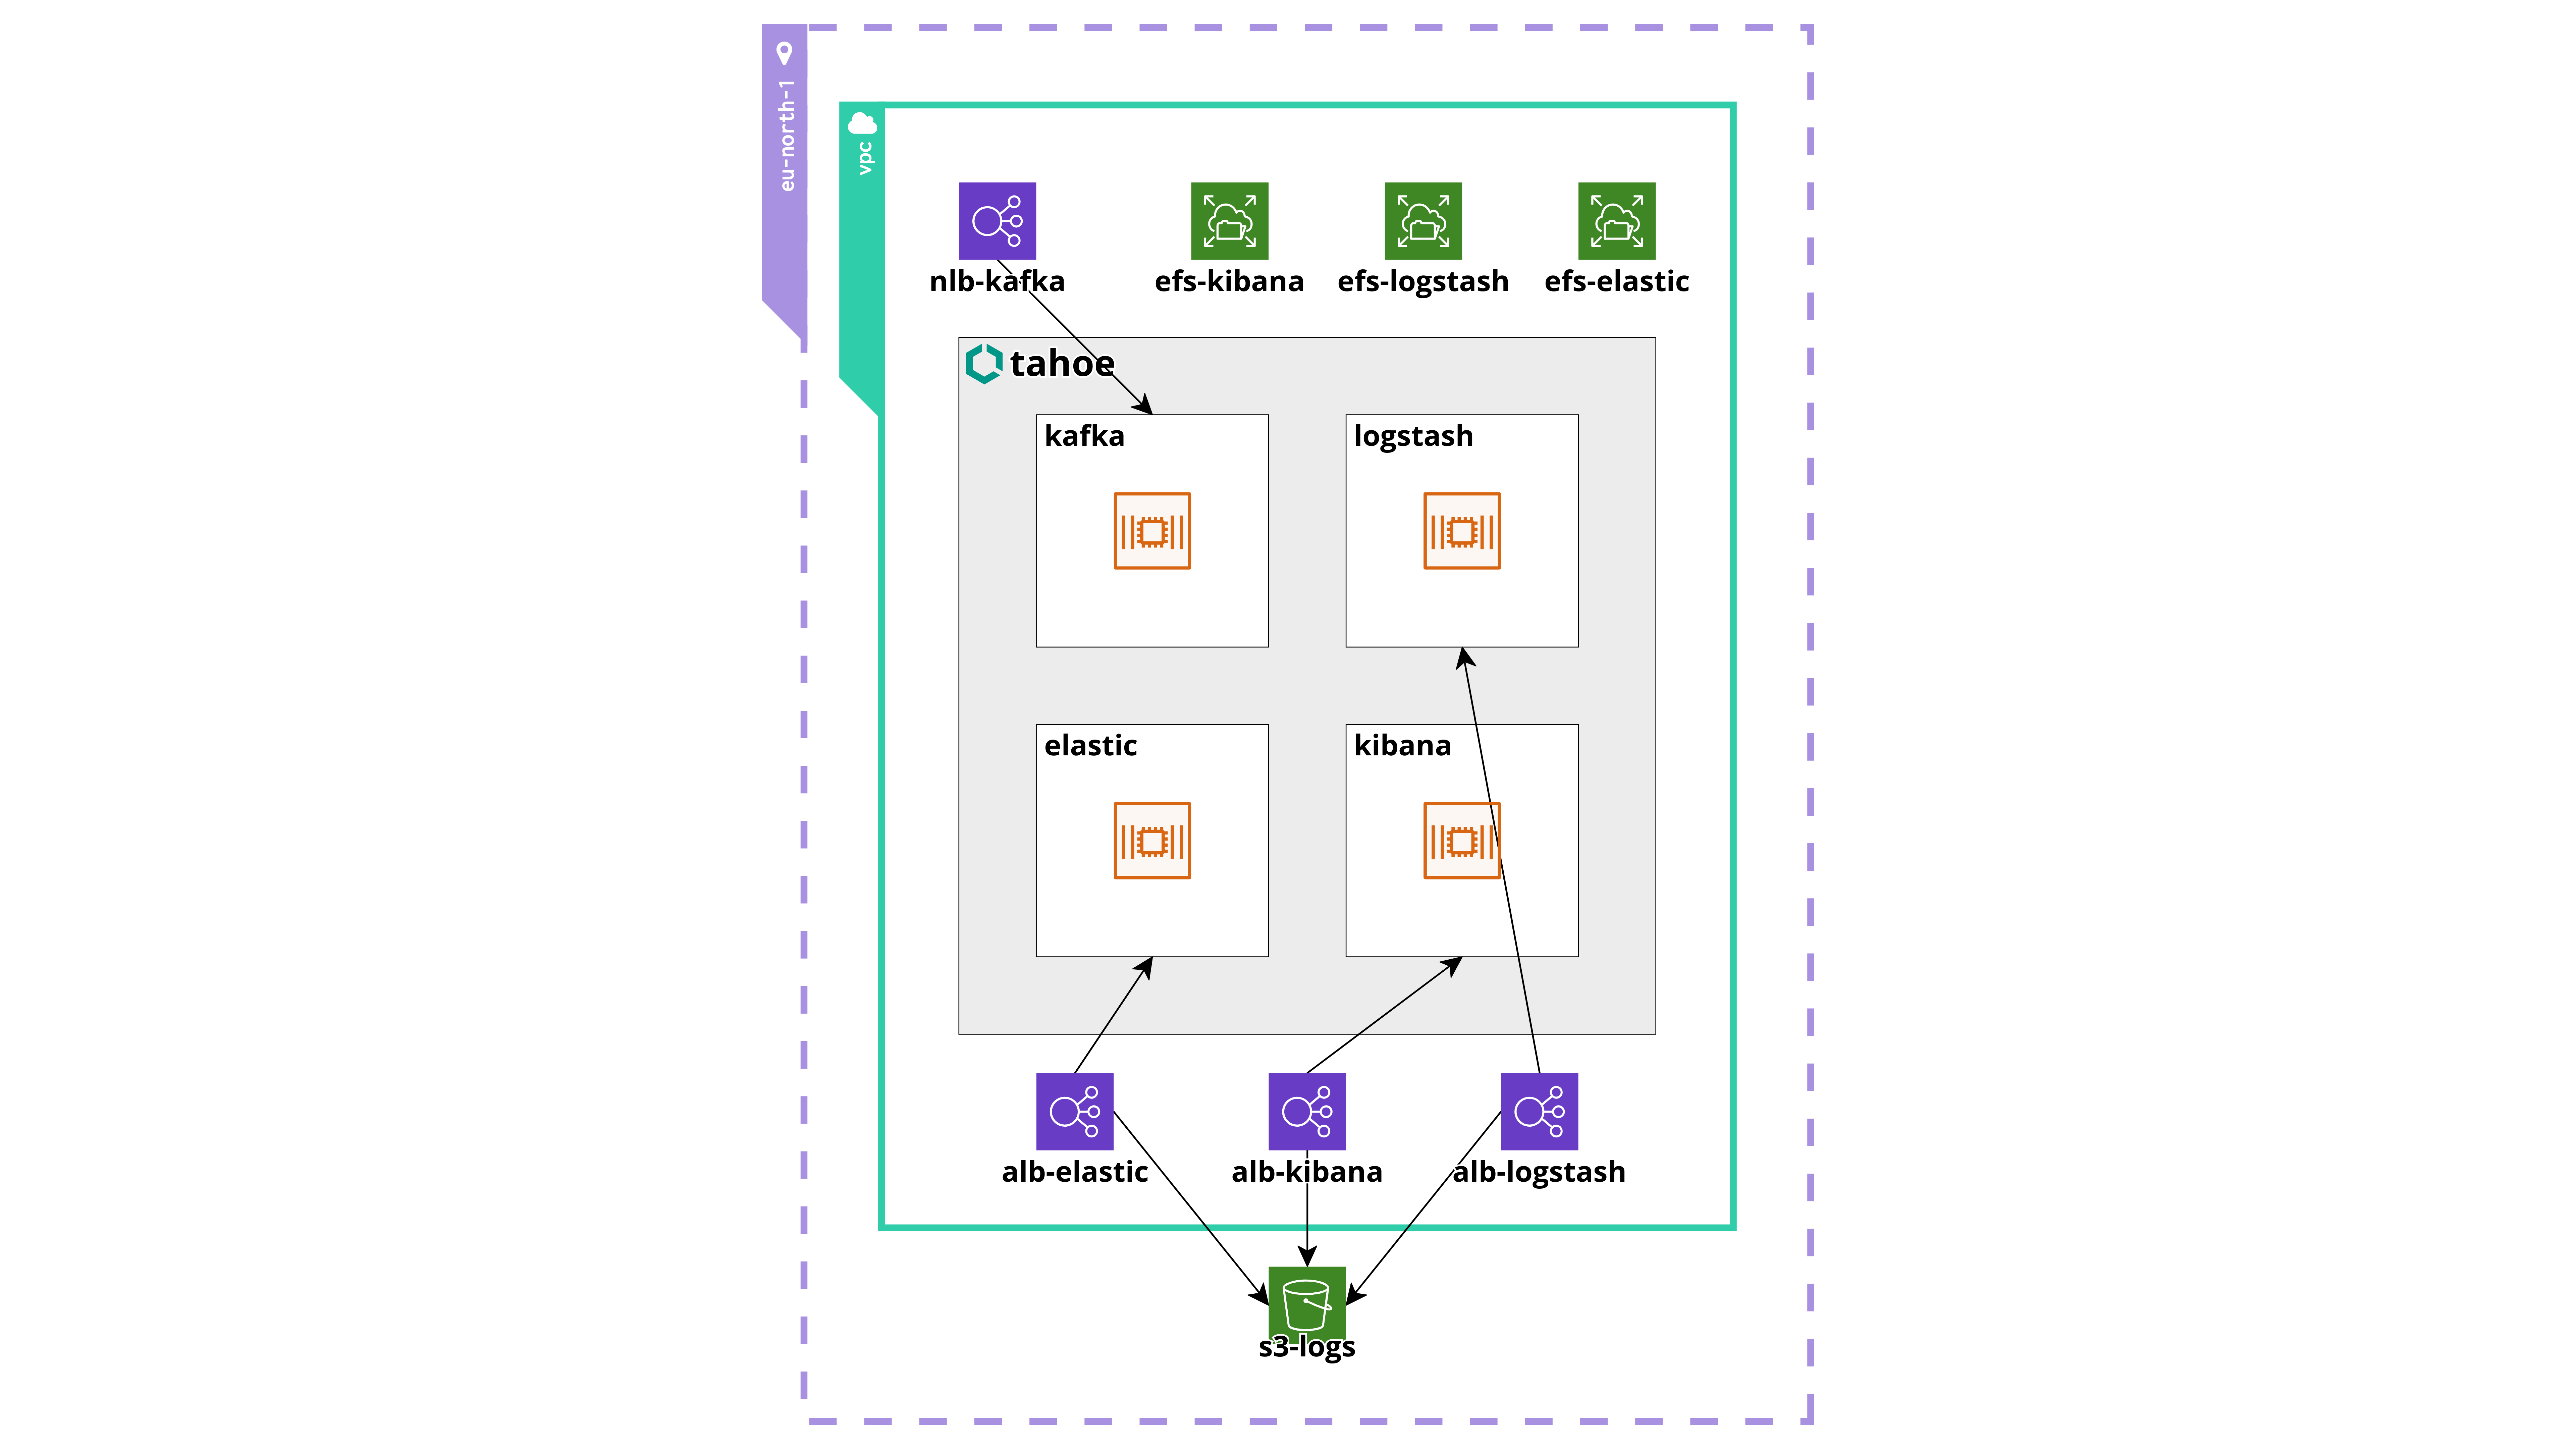
\includegraphics[width=1.3\textwidth]{infra/aws_infra.png}}
	\caption{Diagrama inicial de la infraestructura en AWS}

	\label{fig:aws_infra}
\end{figure}


\subsection{Seguridad}\label{subsec:seguridad}
A nivel de seguridad, se debe garantizar la protección de los datos y la
confidencialidad de la información. Para ello, se utilizarán varios servicios de
AWS, como \textit{IAM} para la gestión de roles y políticas de seguridad, o
\textit{grupos de seguridad} que permiten controlar el tráfico de red entre los
contenedores del sistema.

Cada uno de los componentes del \textit{clúster} de \textit{ECS} tendrá su
propio grupo de seguridad que permitirá controlar el tráfico de red según los
puertos y protocolos permitidos. Además, se deberán utilizar tan solo las
políticas y roles necesarios para garantizar la seguridad de los datos.

Además de los componentes de seguridad de AWS, se utilizarán protocolos seguros
como \textit{HTTPS} para la comunicación entre los servicios y se cifrará la
información haciendo uso de \textit{Secret Manager} para cargar y guardar las
claves necesarias.


\begin{figure}[H]
	\centerline{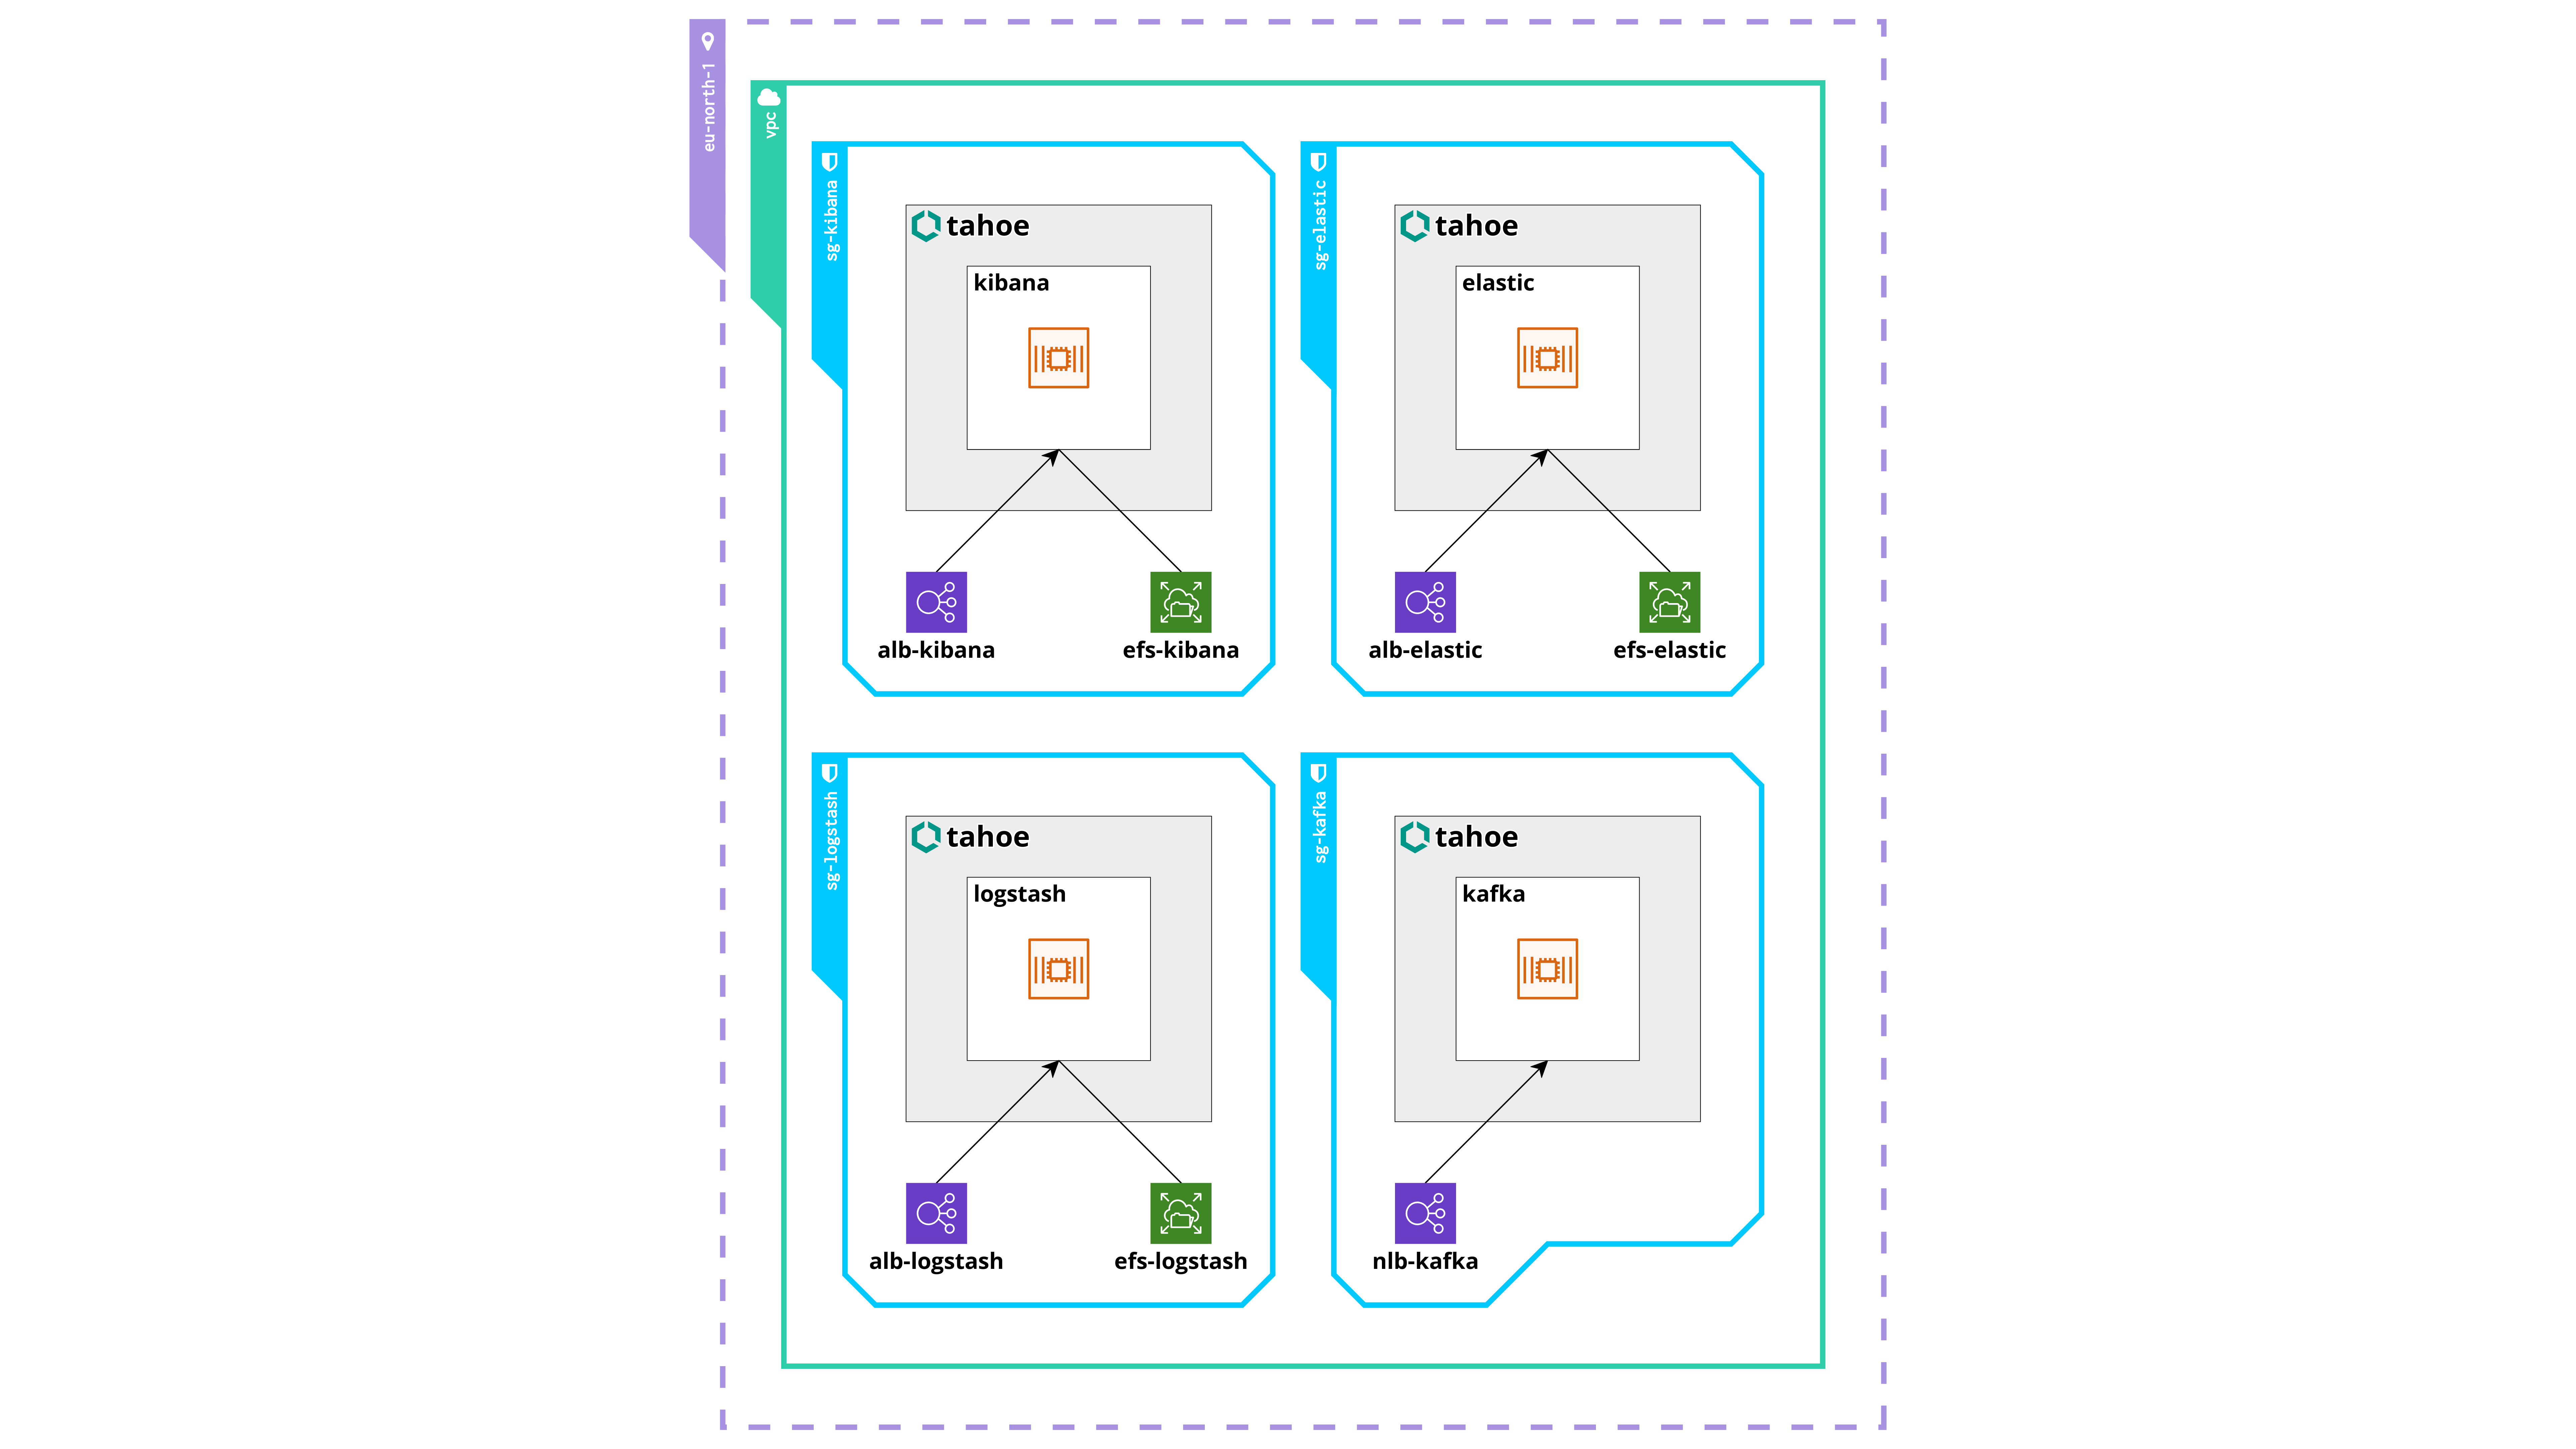
\includegraphics[width=1.3\textwidth]{infra/aws_seguridad.png}}
	\caption{Diagrama incial de la seguridad en AWS}
	\label{fig:aws_seguridad}
\end{figure}

En el diagrama anterior, se pueden observar los grupos de seguridad (resaltados
en azul) que engloban a los componentes, mientras que todos ellos se encuentran
dentro de una \textit{VPC}.

\subsection{Redes}\label{subsec:redes}
A nivel de configuración de redes, se establecen tres subredes: dos públicas y
otra privada, estando las públicas en zonas de disponibilidad diferentes. La
subred pública estará conectada a internet a través de un
\textit{Internet Gateway}, mientras que la subred privada estará conectada a
internet a través de un \textit{NAT Gateway}. Ambas subredes estarán conectadas
a una \textit{VPC} que permitirá la comunicación entre los servicios del
sistema.

\begin{figure}[H]
	\centerline{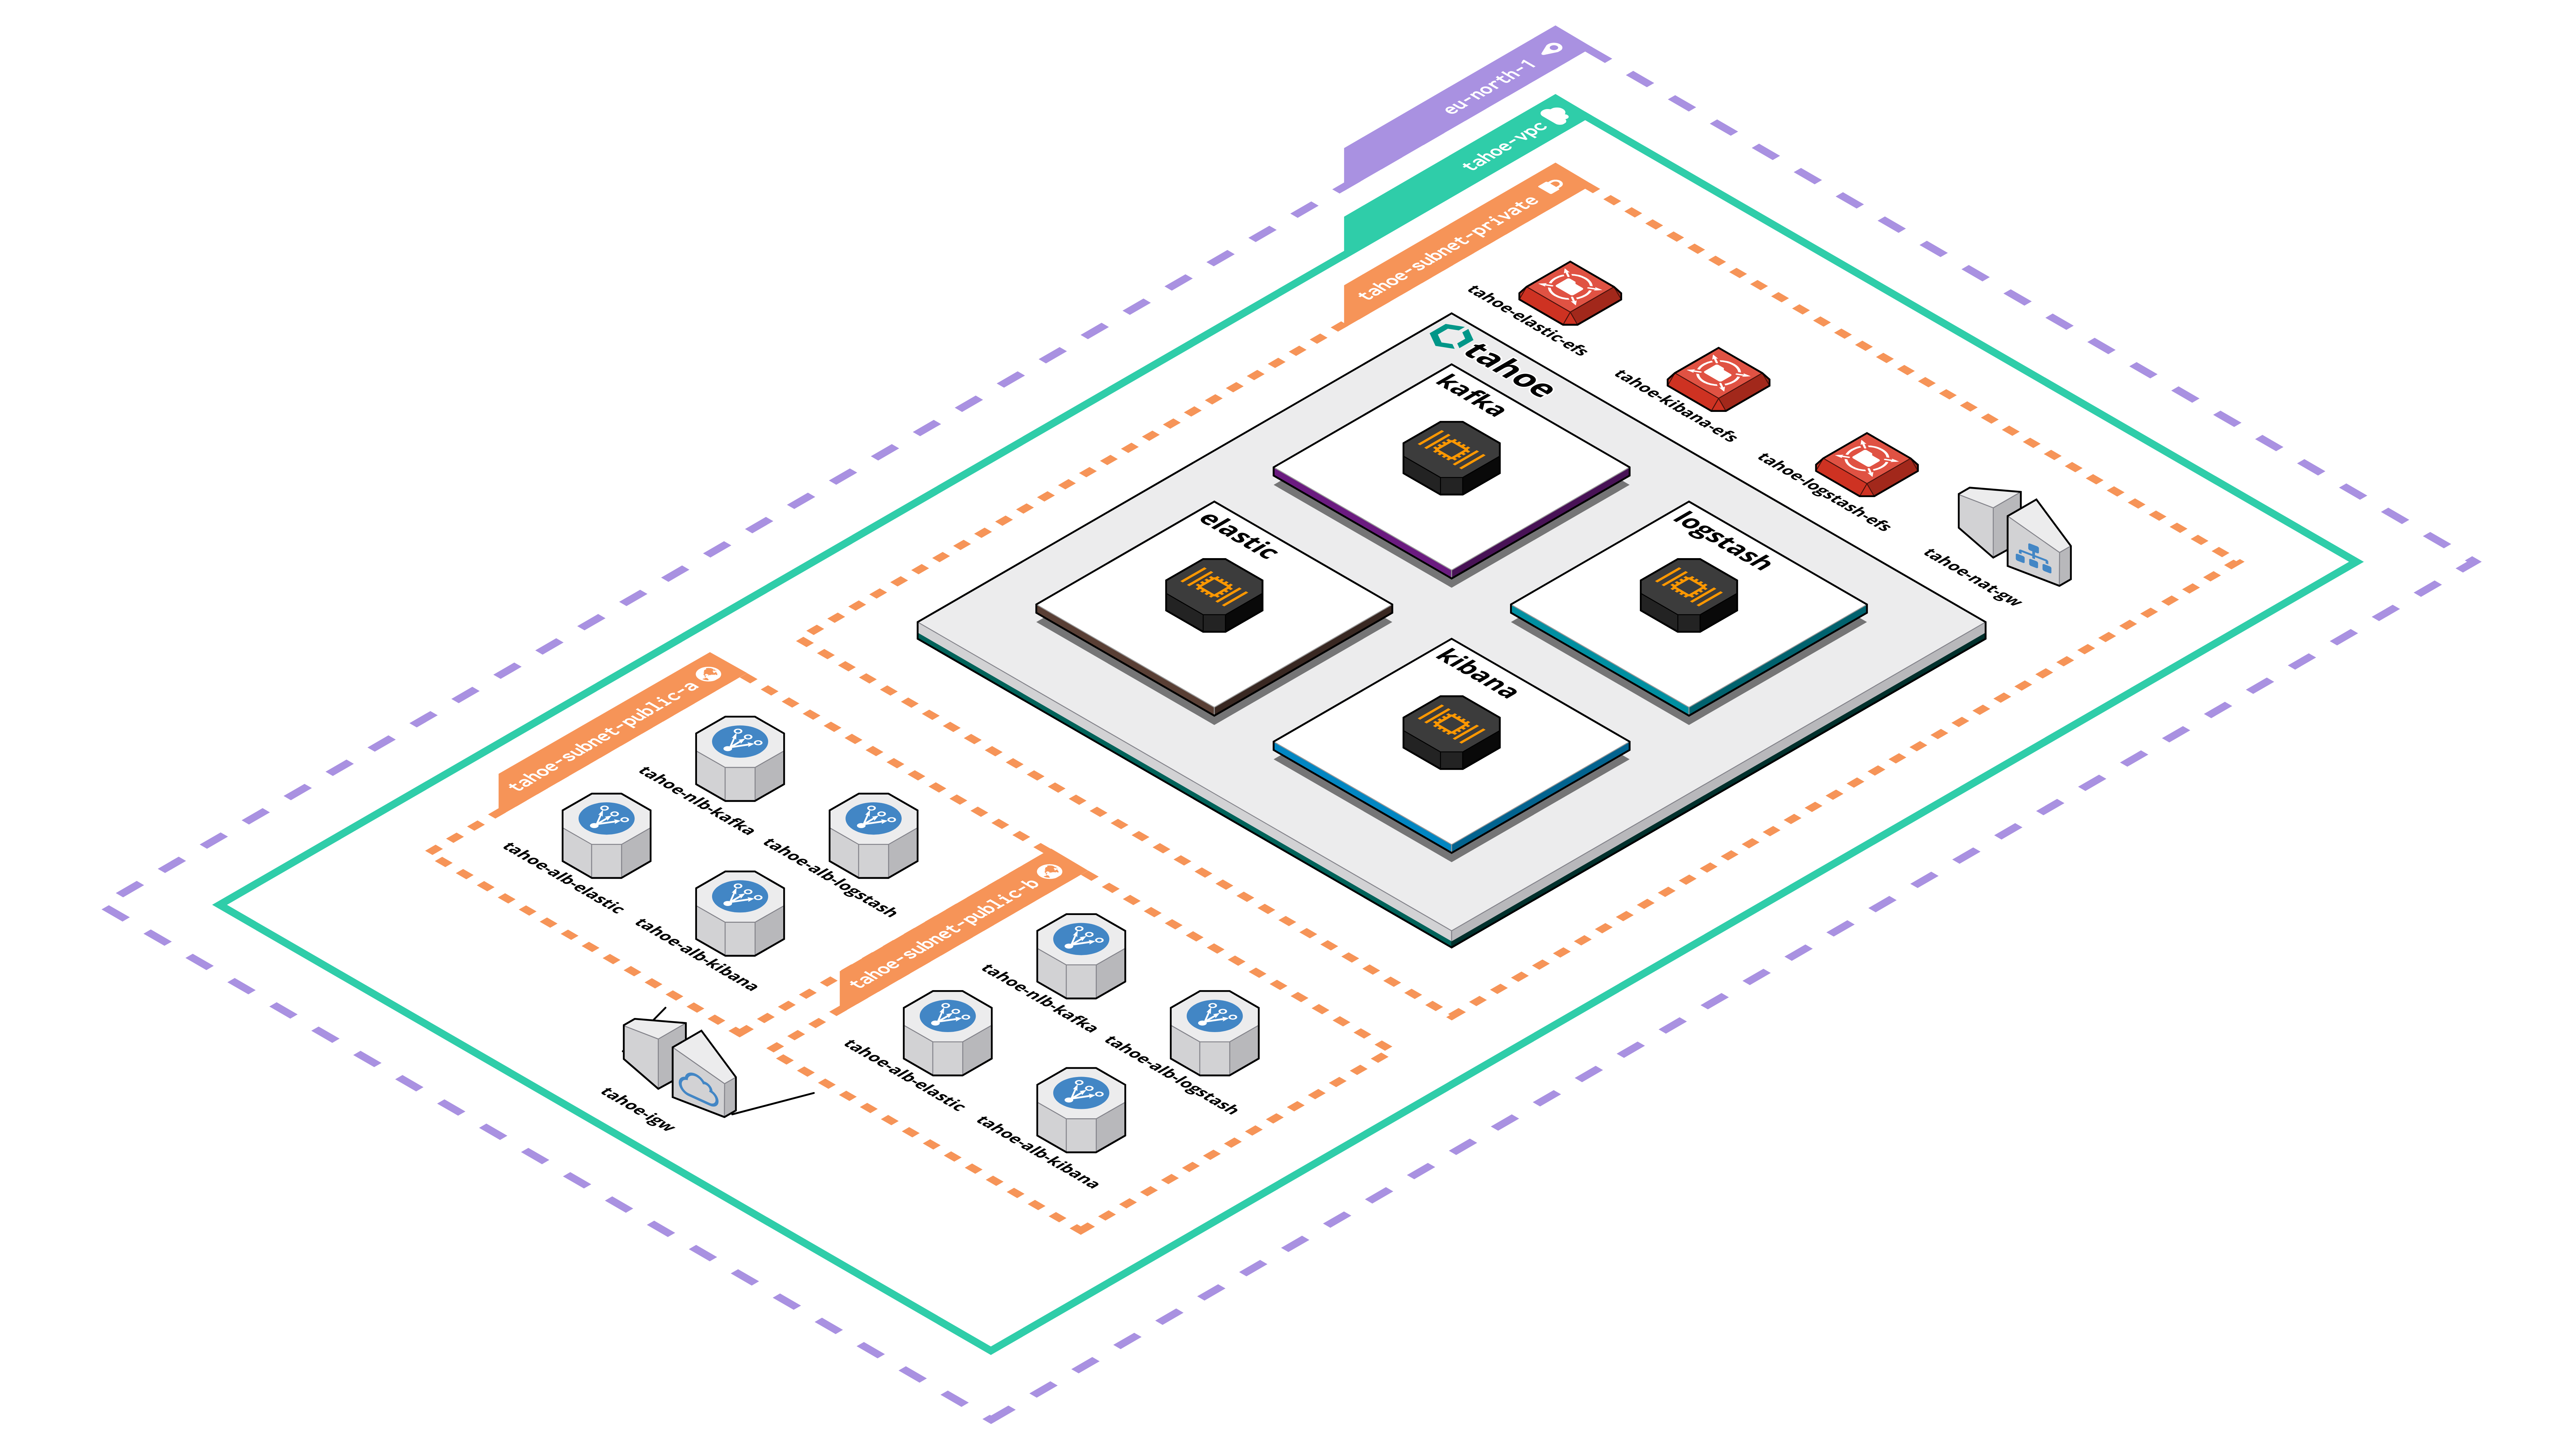
\includegraphics[width=1.3\textwidth]{infra/aws_redes.png}}
	\caption{Diagrama incial de las redes en AWS}
	\label{fig:aws_redes}
\end{figure}

En el diagrama se pueden observar las subredes (resaltadas en naranja con líneas
intermitentes), siendo las dos inferiores subredes públicas en diferentes zonas
de disponibilidad conectadas a un \textit{Internet Gateway} y la subred superior
una privada donde se encuentran los servicios junto con el \textit{NAT Gateway}
necesario para la conexión a Internet.

Además de los componentes planteados en el esquema anterior, se configurarán
\textit{rutas} y \textit{tablas de rutas} para garantizar la conectividad y la
seguridad de los servicios del sistema.
